% !TeX encoding = UTF-8
% !TeX spellcheck = en_US
% !TeX root = slackforceDocumentation.tex

\chapter{Calculate Force} \label{sec:calculateForce}
The forces in a slackline can be obtained by using the geometric setup of the line at a given load. If the tension of the line at a given sag is known the tension at a different sag can easily be calculated with the aid of the stretch behavior.

\section{Basics} \label{sec:basics}

\begin{figure}[htb] \centering
	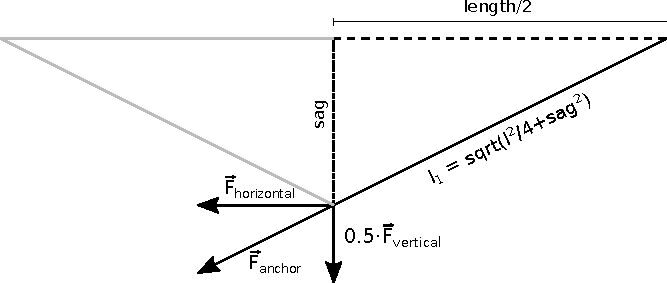
\includegraphics[width=0.8\textwidth]{images/slacklineWithForces.pdf}
	\caption{Schematical slackline with horizontal and vertical components of an applied force}
	\label{fig:slacklineWithForces}
\end{figure}

Figure \ref{fig:slacklineWithForces} shows a scheme of a slackline with a given length and sag. The load that is applied in the middle of the line results in a specific sag. The force on the anchor $F_a$ is determined by the vertical Force $F_v$ and horizontal force $F_h$ as shown in Figure \ref{fig:slacklineWithForces}. The forces on the left part of the line correspond to the shown forces on the right side. The total force is the sum of the forces on the left and the right side. The horizontal components eliminate each other while the vertical ones add up. If a slackliner is standing on the line, the total vertical force corresponds to the slackliner's weight. From the geometric properties shown in figure \ref{fig:slacklineWithForces} the following equation can easily be derived:


\begin{equation}
	\frac{F_a}{0.5\cdot F_v} = \frac{l_1}{s} = \frac{\sqrt{\frac{l^2}{4} + s^2}}{s}
\end{equation}

Together with the gravity acceleration $g = 9.81\frac{m}{s^2}$ and the weight of the slackliner $m$ this leads to the following four equations:

\begin{spreadlines}{1.5\baselineskip}
\begin{align}
	F &= \frac{\sqrt{s^2 + \frac{l^2}{4}}}{2\cdot s} \cdot m\cdot g \label{eqn:calcForce} \\
	m &= \frac{2\cdot s\cdot F}{g\cdot\sqrt{s^2 + \frac{l^2}{4}}} \label{eqn:calcWeight} \\
	s &= \sqrt{ \frac{m^2\cdot l^2\cdot g^2}{4\cdot(4F^2 - m^2g^2)} } \label{eqn:calSag} \\
	l &= \sqrt{ \frac{4\cdot s\cdot (4F^2 - m^2g^2)}{m^2g^2} } \label{eqn:calcLength} 
\end{align}
\end{spreadlines}

With Equation \ref{eqn:calcForce} - \ref{eqn:calcLength} it is possible to calculate any of the parameters force, weight of slackliner, sag and length, if the other parameters are known.

\section{Calculating the Pretension}

\begin{figure}[htb] \centering
	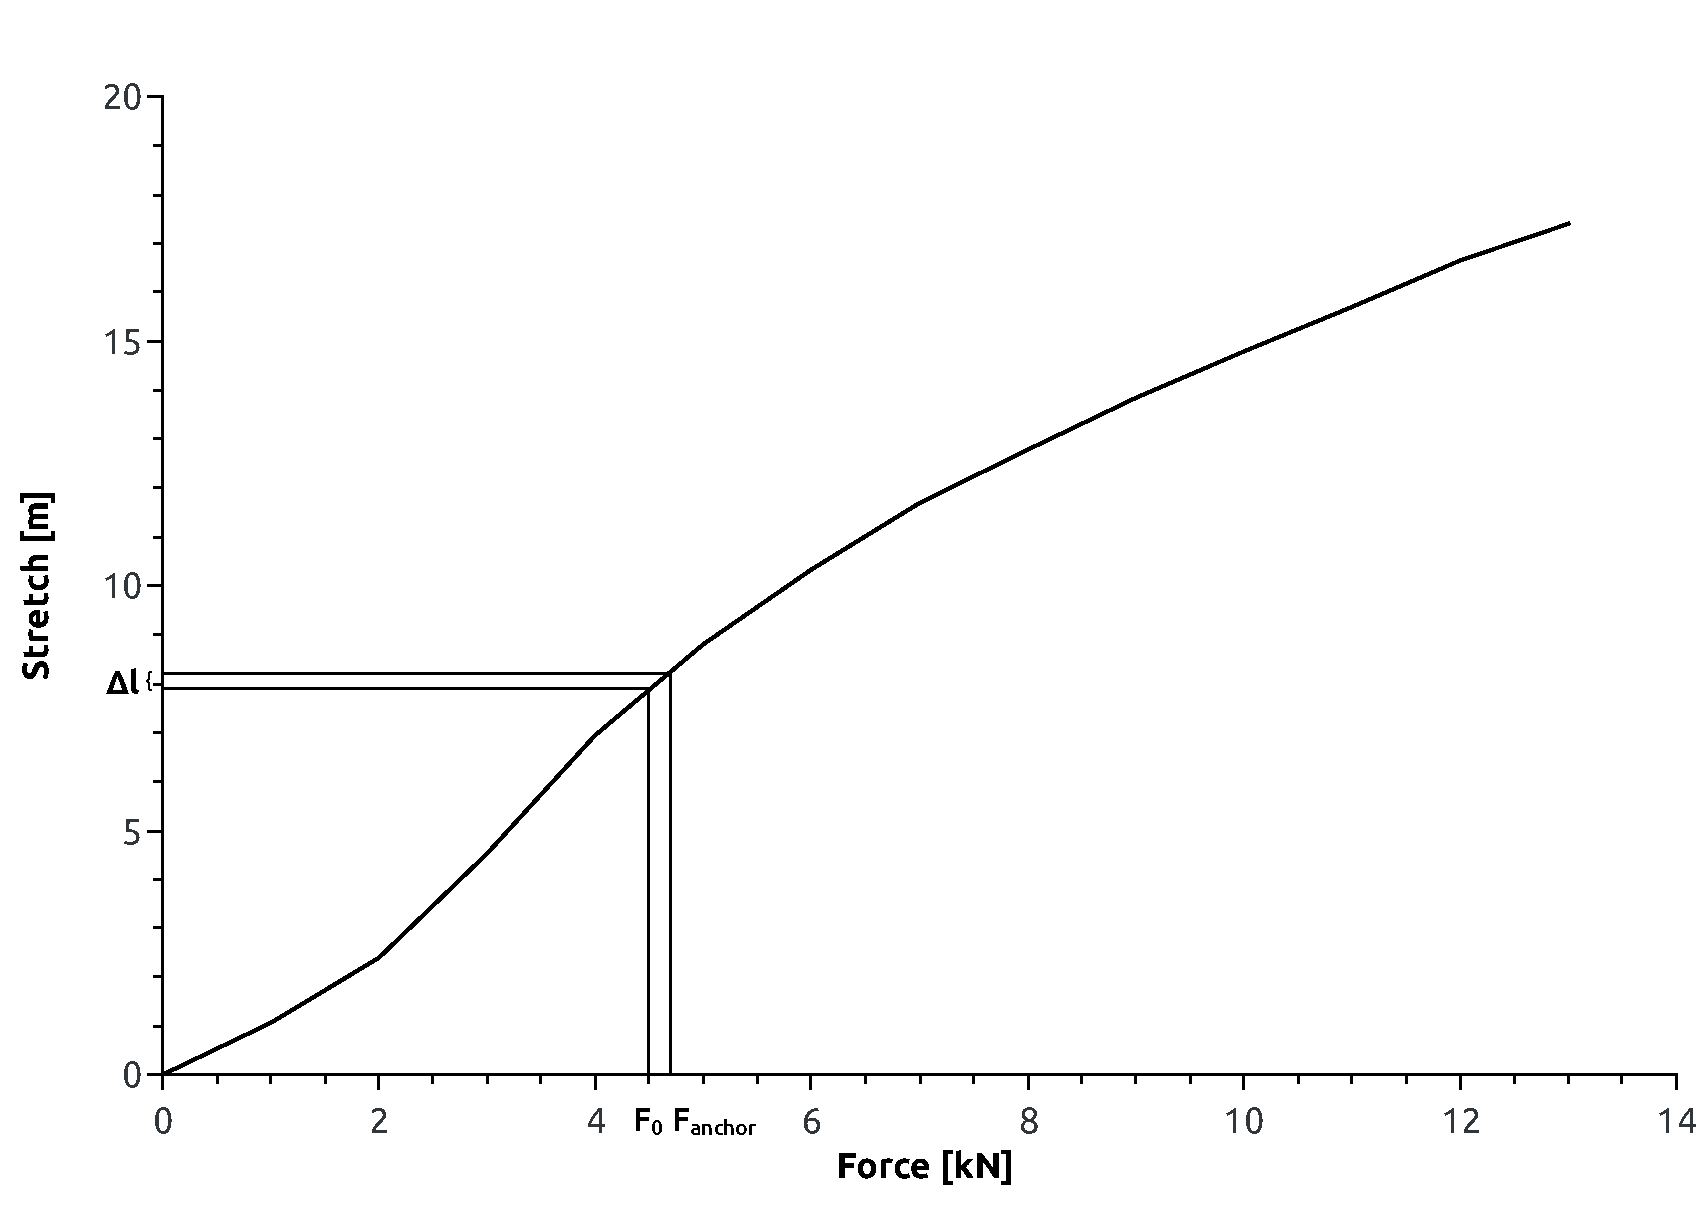
\includegraphics[width=0.8\textwidth]{images/forceStretchDiagram.pdf}
	\caption{Force-Stretch-Diagramm of a 100\,m Type 18 Line with 4,5\,kN Pretension}
	\label{fig:forceStretchDiagramm}
\end{figure}

If you know the (walking) tension of a slackline with a person standing in the middle and the stretch behavior, it is possible to calculate the pretension. Figure \ref{fig:forceStretchDiagramm} shows the stretch behavior of a Type 18 MKII line as an example. It can be seen that the stretch is not linear. To get the pretension of the line you need to know the increase of length $\Delta l$ due to the sag of the line. This can be calculated with the following formula:

\begin{equation}
	\Delta l = 2\cdot l_1 - l= 2\cdot \sqrt{s^2+\frac{l^2}{4}} - l
	\label{eqn:deltaL}
\end{equation}

To get the pretension you have to do the following steps:

\begin{enumerate}
	\item Calculate the anchor force with a slackliner on the line
	\item Read the corresponding stretch from the force-stretch-diagram
	\item Calculate the new stretch with formula \ref{eqn:deltaL}
	\item Read the pretension from the force-stretch-diagram
\end{enumerate}

If a linear stretch behavior $\frac{\Delta l}{l} = \alpha\cdot F$ is assumed, it is possible to put that relation into an analytic formula:

\begin{equation}
	F = F_0 + \frac{2\cdot \sqrt{s^2+\frac{l^2}{4}} - l}{\alpha\cdot l}
\end{equation}

However, the app always uses the force-stretch-diagram if available, as the results are better with that method.  Unfortunately some slackline manufacturers provide very little information on the stretch behavior of their lines and only a few data points are available. The app interpolates those data points linear for the calculations.

\section{Rodeo Lines}

Rodeo Lines are slacklines with a lot of sag and no pretension. So the pretension $F_0$ is always zero and the line has an initial sag $s_0$ without any slackliner standing on the line. When a slackliner steps on the line, it might stretch further and lead to a sag greater than the initial sag. Figure \ref{fig:RodeoLineWithForces} shows the forces on an rodeo line.

\begin{figure}[htb] \centering
	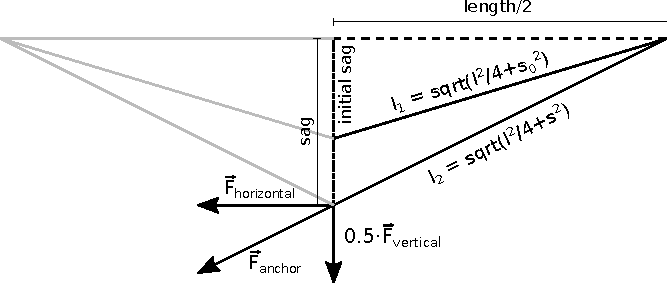
\includegraphics[width=0.8\textwidth]{images/rodeoLineWithForces.pdf}
	\caption{Schematical rodeo line with horizontal and vertical components of force}
	\label{fig:RodeoLineWithForces}
\end{figure}

As it can be seen there is no change to the static forces with a slackliner on the line from figure \ref{fig:slacklineWithForces}. So all the calculations of the section ``\nameref{sec:basics}'' are still valid. If you want to do calculations based on the force-stretch-diagram you have to be aware that equation \ref{eqn:deltaL} now changes to

\begin{equation}
	\Delta l = 2\cdot (l_2 - l_1) = 2\cdot \left( \sqrt{s^2+\frac{l^2}{4}} - \sqrt{s_0^2+\frac{l^2}{4}}\right)
	\label{eqn:deltaLRodeo}
\end{equation}

In addition there is no pretension to calculate, but you can calculate the initial sag of the line using the force-stretch-diagram. Therefore you have to read the stretch $\Delta l$ from the diagram and use the following formula:

\begin{align}
	s_0 &= \sqrt{l_1^2 - \frac{l^2}{4}} = \sqrt{\left(l_2-\Delta l\right)^2 - \frac{l^2}{4}} \\
	&= \sqrt{\left( \sqrt{s^2 + \frac{l^2}{4}}  -\Delta l\right)^2 - \frac{l^2}{4}}
\end{align}

\section{Calculating Slackline Forces from the Pretension}

Unfortunately it is very difficult for linear stretch behavior and impossible for a custom stretch behavior to get an analytic expression of the walking tension, that is a function of the pretension. Therefore some kind of approximation algorithm has to be used. The App is currently using the Illinois algorithm.

\section{Slackliner who is not in the middle of the Line (not implemented)}

In the following it is assumed, that the slackliner is standing at a position $p \in [0,1]$ on the line. The forces are always calculated for the left anchor point. The forces at the right anchor point equal the forces at the left anchor point at position $1-p$. Figure \ref{fig:slacklineWithForcesUnsymmetric} shows the forces in this new setup. If the slackliner is not moving, the horizontal forces have to be the same on both sides. That leads to different vertical forces and anchor forces on both sides.

\begin{figure}[htb] \centering
	\begin{subfigure}{\textwidth} \centering
		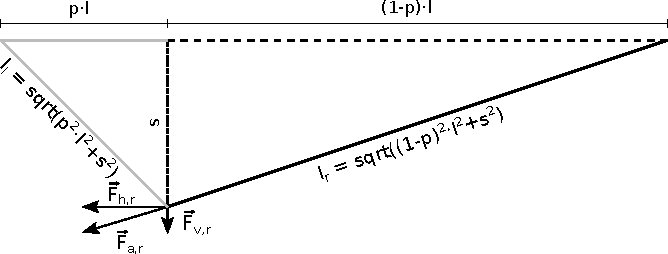
\includegraphics[width=0.8\textwidth]{images/slacklineWithForcesUnsymmetricRightSide.pdf}
	\end{subfigure} \par\bigskip
	\begin{subfigure}{\textwidth} \centering
		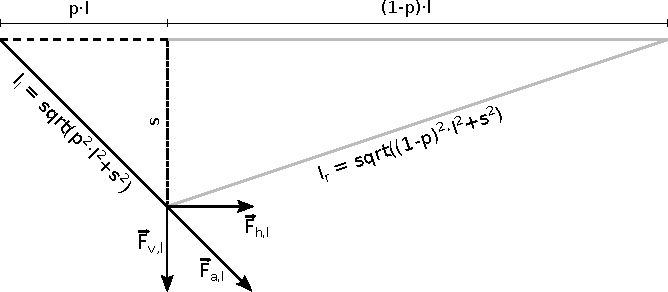
\includegraphics[width=0.8\textwidth]{images/slacklineWithForcesUnsymmetricLeftSide.pdf}
	\end{subfigure}
	\caption{Force Components on Unsymmetric Conditions }
	\label{fig:slacklineWithForcesUnsymmetric}
\end{figure}

According to fig. \ref{fig:slacklineWithForcesUnsymmetric} the equation below can be derived.

\begin{equation}
	\frac{p\cdot l}{s} = \frac{F_{h,l}}{F_{v,l}} = \frac{ \sqrt{F_{a,l}^2 - F_{v,l}^2 }}{F_{v,l}}
	\label{eqn:geometricPropertiesUnsymmetric}
\end{equation}

The total vertical force is still the sum of both sides:

\begin{equation}
	F_v = F_{v,l} + F_{v,r}
	\label{eqn:verticalForce}
\end{equation}

The absolute values of both horizontal forces are the same which leads to:

\begin{equation}
	\frac{p\cdot l}{s}\cdot F_{v,l} = \frac{(1-p)\cdot l}{s}\cdot F_{v,r} 
	\label{eqn:horizontalEquality}
\end{equation}

Combining equation \ref{eqn:horizontalEquality} and \ref{eqn:verticalForce} results in:

\begin{equation}
	F_{v,l} = (1-p)\cdot F_v
	\label{eqn:leftVerticalForce}
\end{equation}

Inserting equation \ref{eqn:leftVerticalForce} in \ref{eqn:geometricPropertiesUnsymmetric} leads to the final equation

\begin{equation}
	F_{a,l} = \frac{(1-p)\cdot F_v}{s}\cdot \sqrt{(p\cdot l)^2 + s^2}
\end{equation}

For $p = 0.5$ this equation is identical to equation \ref{eqn:calcForce} from the previous section. Note that equation \ref{eqn:deltaL} now changes to

\begin{equation}
	\Delta l = \sqrt{ (p\cdot l)^2 + s^2 } + \sqrt{ (1-p)^2 l^2 + s^2 } - l
\end{equation}






